

%\input{"F:/Dropbox/FlashDrive-64GB/CalPoly-prof/STAT331/Glanz/Spring2018/Notes/SlideStyleR.tex"}
\input{"C:/Users/hglanz/Dropbox/Hunter/FlashDrive-64GB/CalPoly-prof/STAT331/Glanz/Spring2018/Notes/SlideStyleR.tex"}


\title[]{Introduction to Linear Models \\
									(Regression)}
\author[Glanz]{Hunter Glanz}

%\institute[BUS 450]{BUS 450}

\date{}


\begin{document}

\begin{frame}
\titlepage
\end{frame}

\begin{frame}
\frametitle{OUTLINE\qquad\qquad\qquad} \tableofcontents[hideallsubsections]
\end{frame}


%===========================================================================================================================
\section[Motivation]{Motivation}
%===========================================================================================================================

\subsection{}

\begin{frame}
\frametitle{Data Exploration to Data Analysis}
\bi
	\item What are the observations?
	\item What variables do we have?
	\pause
	\item What are the values of these variables like?
	\pause
	\item What kinds of relationships are there among the variables we have?
	\pause
\ei
\begin{center}
	\textbf{Storytelling with data!}
\end{center}
\end{frame}

\begin{frame}
\frametitle{The Carseats Dataset in the ISLR package for R}
\bi
	\item 400 observations on the following variables:
	\bi
		\item Sales (in thousands) at each location
		\item CompPrice
		\item Income
		\item Advertising
		\item Population
		\item Price
		\item ShelveLoc
		\item Age
		\item Education
		\item Urban
		\item US
	\ei
	\item More info here: \url{https://rdrr.io/cran/ISLR/man/Carseats.html}
\ei
\end{frame}

\begin{frame}
\frametitle{Research Questions}
\bi
	\item What kinds of questions might you ask of this dataset?
	\item What kinds of questions might have caused you to collect/obtain these data?
	\pause
	\item Primary question:
\ei

\pause

\begin{center}
	\textbf{Can we predict Sales using the other information in this dataset?}
\end{center}
\end{frame}

%===========================================================================================================================
\section[Univariate]{Univariate}
%===========================================================================================================================

\subsection{}

\begin{frame}[fragile]
\ft{What do we know about Sales?}
\begin{center}
	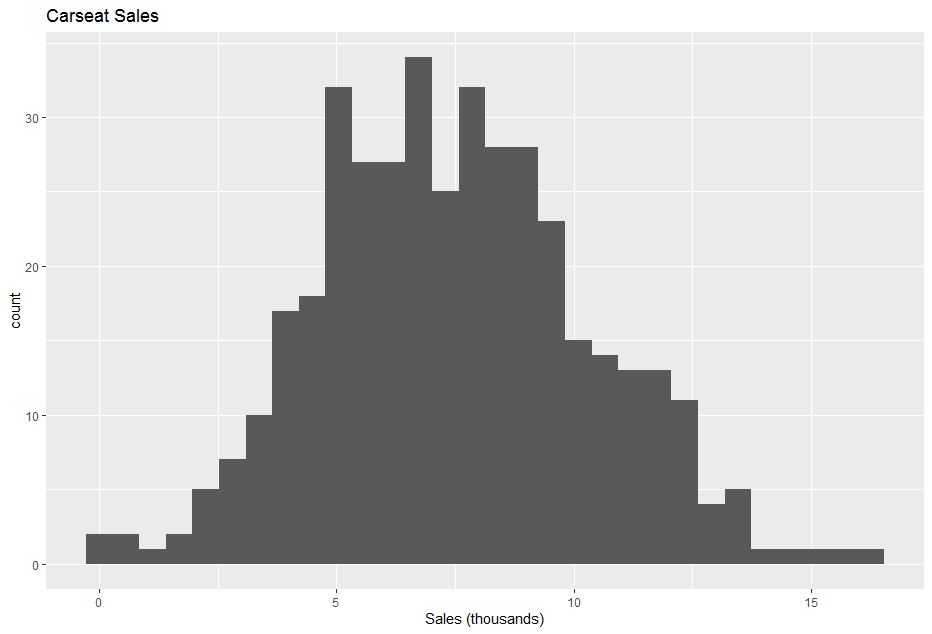
\includegraphics[width = 4in]{SalesHist.png} \\
	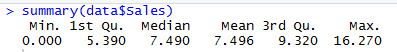
\includegraphics[width = 2in]{SalesSumm.png}
\end{center}

\end{frame}

\begin{frame}
\ft{Other Possible Visualizations...?}
\pause
\begin{center}
	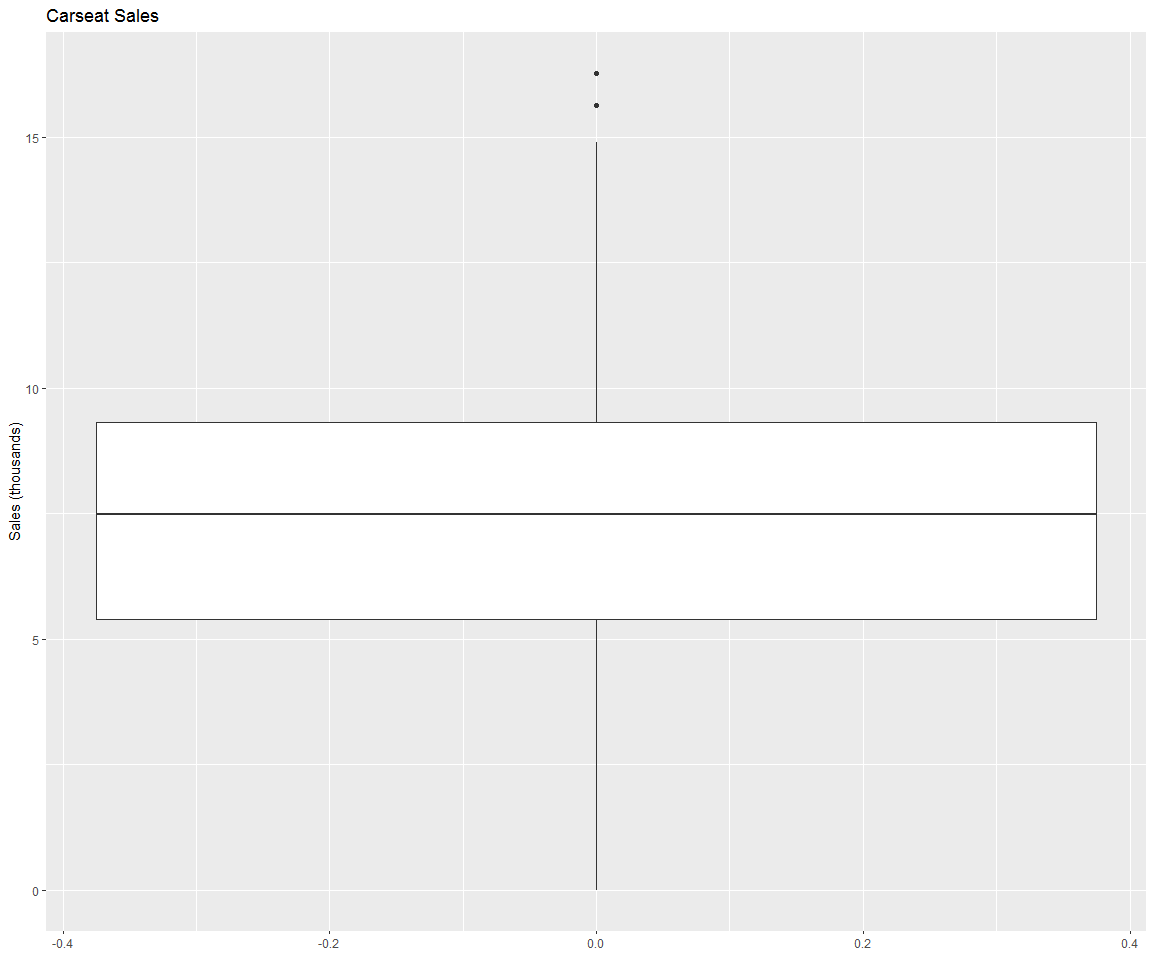
\includegraphics[width = 3in]{SalesBox.png}
\end{center}
\end{frame}

\begin{frame}
\ft{Another Visualization?}
\begin{center}
	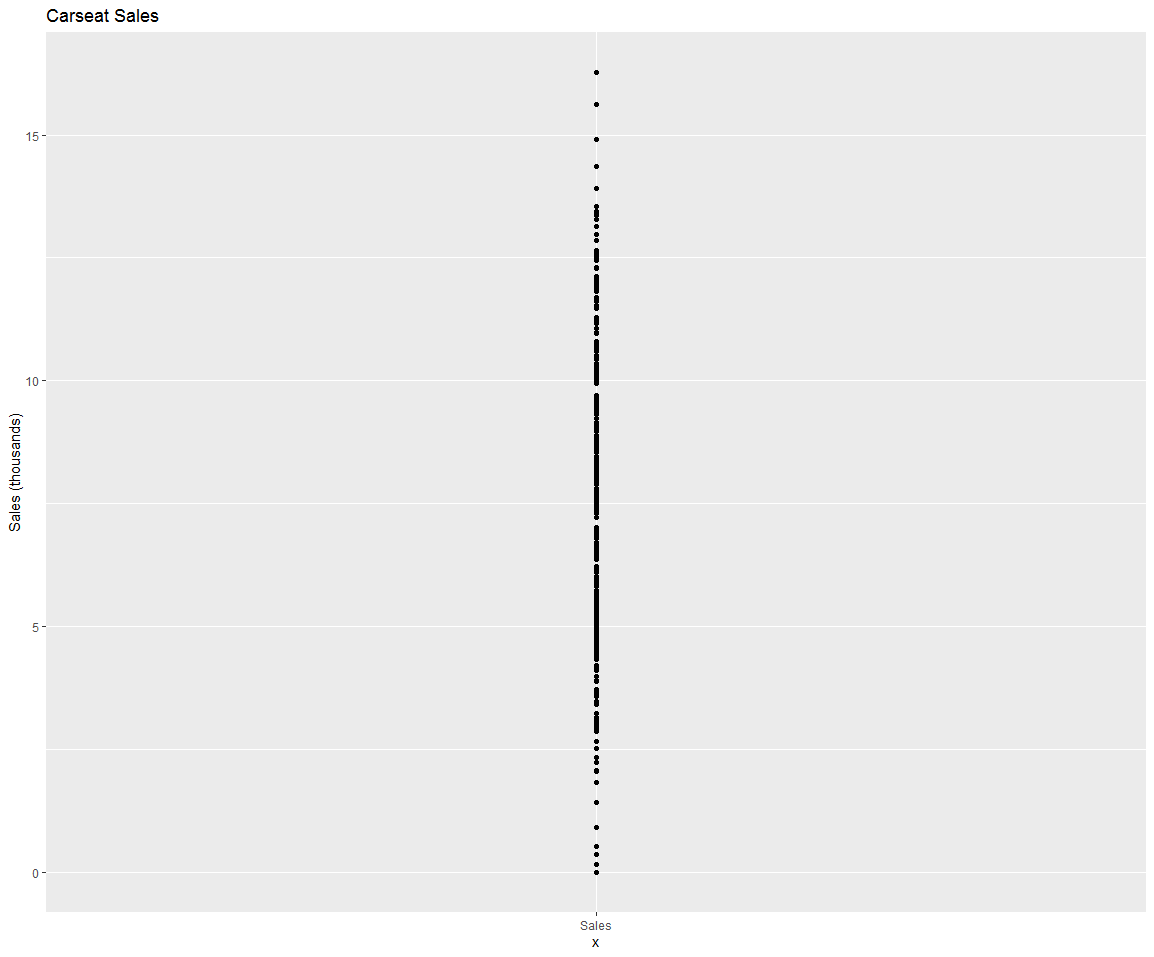
\includegraphics[width = 3in]{SalesPoints.png}
\end{center}
\end{frame}

\begin{frame}
\ft{Another Visualization? With the Mean...}
\begin{center}
	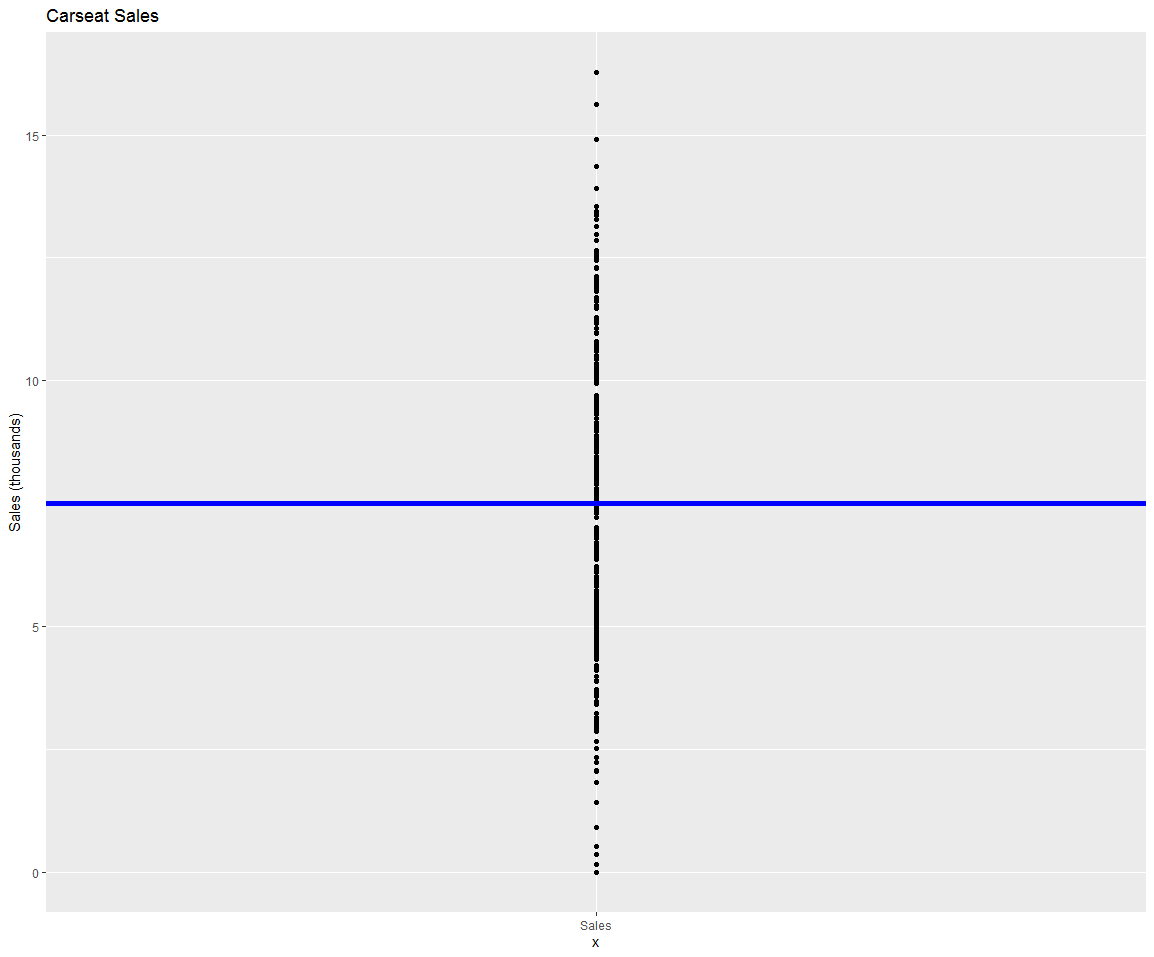
\includegraphics[width = 3in]{SalesPointsMean.png}
\end{center}
\end{frame}

\begin{frame}
\ft{Predicting Sales Part I}
\bi
	\item Without knowing any other information or using any other data, what would your prediction for Sales be?
	\pause
		\bi
			\item The most representative value of Sales that we have access to, right?!
		\ei
	\pause
	
	\item The mean or average of Sales is a good start: 7.5 thousand
\ei
\end{frame}


%\begin{frame}
%\frametitle{A Few Quick Notes}
%\bi
%\item A package only needs to be installed once per machine.
%\item A package needs to be loaded in every R session it's going to be used.
%\item The package name needs to be in quotes when installing it.
%\item R is \textbf{case-sensitive}, so typing \texttt{library(ISWR)} will not work.
%\ei
%\end{frame}
%
%\begin{frame}
%\frametitle{Basic Math, Functions, and Operators}
%\bi
%\item You can type directly into the console to do basic math operations. Try the following in the console (one at a time):
%\bi
%\item $2+2$
%\item $6^3$
%\item $25*10$
%\item $16-2*4$
%\ei
%\item Notice the default prompt of ``$>$" means that R is ready for new instructions (i.e. for you to enter code). 
%\ei
%\end{frame}
%
%\begin{frame}
%\begin{clicker}{What if you entered ``2+" in the console and hit enter. What would you see?}
%\begin{enumerate}
    %\item Nothing would be computed
    %\item An error since the operation is incomplete
    %\item 2
    %\item A new prompt indicating R is waiting for more
%\end{enumerate}
%\end{clicker}
%
%\bi
%\item Try it!
%\ei
%\end{frame}
%
%\begin{frame}
%\ft{RStudio's Panels}
%\bi
	%\item Four primary panels: Console, Script, Environment, Plots/Misc.
	%\begin{enumerate}
		%\item \textbf{Console}: this is where we've been!
		%\item \textbf{Script}: A place to write code without immediately executing it
		%\item \textbf{Environment}: A place to see variables and functions
		%\item \textbf{Plots/Misc.}: A place to see plots, packages, help docs
	%\end{enumerate}
%
	%\item \textbf{Script}: File $\rightarrow$ New File $\rightarrow$ R Script
		%\bi
			%\item This is where you'll work with R Notebooks too!
		%\ei
%\ei
%\end{frame}
%
%\begin{frame}[fragile]
%\ft{R Programs I}
%Enter the following code in your R script:
%\bmp{1.0\textwidth}
%\footnotesize
%\begin{code}{.0}
%rnorm(15) \#\# Generate 15 random values from a standard normal dist.
%v <- rnorm(15) \#\# Assign them to a variable named v
%v
%\end{code}
%\emp
%
%\bi
	%\item A hash symbol (\texttt{\#}) denotes a comment. All code to the right will be ignored.
	%\item Line(s) of code can be run using Ctrl + Enter or hitting ``Run" in the upper right of the Script panel.
%\ei
%\end{frame}
%
%
%\begin{frame}[fragile]
%\fto
%\bi
	%\item Copy the following code into your script and run it:
%\bmp{1.0\textwidth}
%\footnotesize
%\begin{code}{.0}
%height <- c(1.75, 1.8, 1.65, 1.90, 1.74, 1.91)
%weight <- c(60, 72, 57, 90, 95, 72)
%plot(height, weight)
%\end{code}
%\emp
	%\item We used \texttt{rnorm()} to create a vector of values before, but we can use \texttt{c()} as well!
%\ei
%\end{frame}
%
%\begin{frame}
%\begin{clicker}{Suppose we want to create a variable for BMI using the formula $BMI = height/weight^2$. How should we do this?}
%\begin{enumerate}
    %\item $c(height[1]/weight[1]^2, height[2]/weight[2]^2, ...)$
    %\item $height/weight^2$
    %\item Use a loop
    %\item On our calculator and then enter the values ourselves, like we did height above
%\end{enumerate}
%\end{clicker}
%\end{frame}
%
%\begin{frame}
%\fto
%\bi
 %\item The \texttt{length()} function returns the number of elements in its input. The \texttt{sum()} function returns the sum of the elements in a vector. \emph{\textbf{Do the following:}}
		%\bi
			%\item Create the BMI vector using the formula on the previous slide.
				%\bi
					%\item Vectorization!!!
				%\ei
			%\item Compute the means of the height, weight, and BMI vectors.
			%\item Try out the \texttt{median}, \texttt{mean}, \texttt{min}, \texttt{max}, and \texttt{round} functions.
		%\ei
%\ei
%\end{frame}
%
%\begin{frame}
%\ft{Getting Help}
%\bi
	%\item To get details on how to use R commands/functions, type \texttt{?[command name]} at the console.
		%\bi
			%\item For example, \texttt{?round}
		%\ei
	%\item For operators, use quotes:
		%\bi
			%\item \texttt{?">="}
		%\ei
		%
	%\item A help page will pull up:
		%\bi
			%\item Description
			%\item Usage
			%\item Arguments
			%\item Details
			%\item Value
			%\item Examples
			%\item A few other things
		%\ei
%\ei
%\end{frame}
%
%
%\begin{frame}
%\ft{If You're Lost}
%\bi
	%\item You may not know the exact command to look for
		%\bi
			%\item \ttp{help.search("keyword")}
			%\item For example, \ttp{help.search("standard deviation")} and then proceed to \ttp{?sd}
		%\ei
			%
	%\item \url{http://www.rseek.org}
	%\item Google
	%\item StackOverflow
%\ei
%\end{frame}
%
%\begin{frame}
%\ft{Saving Your Work}
%\bi
	%\item \ttp{R} is an \emph{object-oriented} programming language -- we create \emph{objects} which are stored in working memory, called the \emph{workspace}.
		%\bi
			%\item To see the workspace, type \ttp{ls()} or just view the \ttb{Environment} panel.
		%\ei
	%\item Notice a save icon at the top of both the \ttb{Script} and the \ttb{Environment} panels. 
		%\bi
			%\item \ttb{Script}: This will save whatever file you have open in the script panel
			%\item \ttb{Environment}: This will save the state of your workspace -- the variables and their values, and any functions you've created.
		%\ei
	%
	%\item You can also save your code history (\ttb{History} tab) and graphs (\ttb{Plots} panel).
%
%\ei
%\end{frame}
%
%\begin{frame}
%\ft{Using R Markdown for Reports}
%\bi
	%\item R Markdown/Notebooks are different than R scripts since they can include markdown text too!
	%\item R code gets written and run in \emph{R code chunks}
		%\bi
			%\item These chunks can be run using the little play symbol in the top right corner of the chunk (or using Ctrl+Enter).
			%\item Results appear just below the chunk
		%\ei
	%\item Anything outside a code chunk is regular/markdown text.
	%
	%\item When you're done, you can \ttt{knit} the markdown/notebook to either a PDF or HTML document.
%\ei
%\end{frame}

%===========================================================================================================================
\section[Bivariate]{Bivariate}
%===========================================================================================================================

\subsection{}

\begin{frame}
\ft{But we DO have more data!}
\bi
	\item Does knowing whether a store is in the U.S. or not help in predicting Sales?
\ei
\pause
\begin{center}
	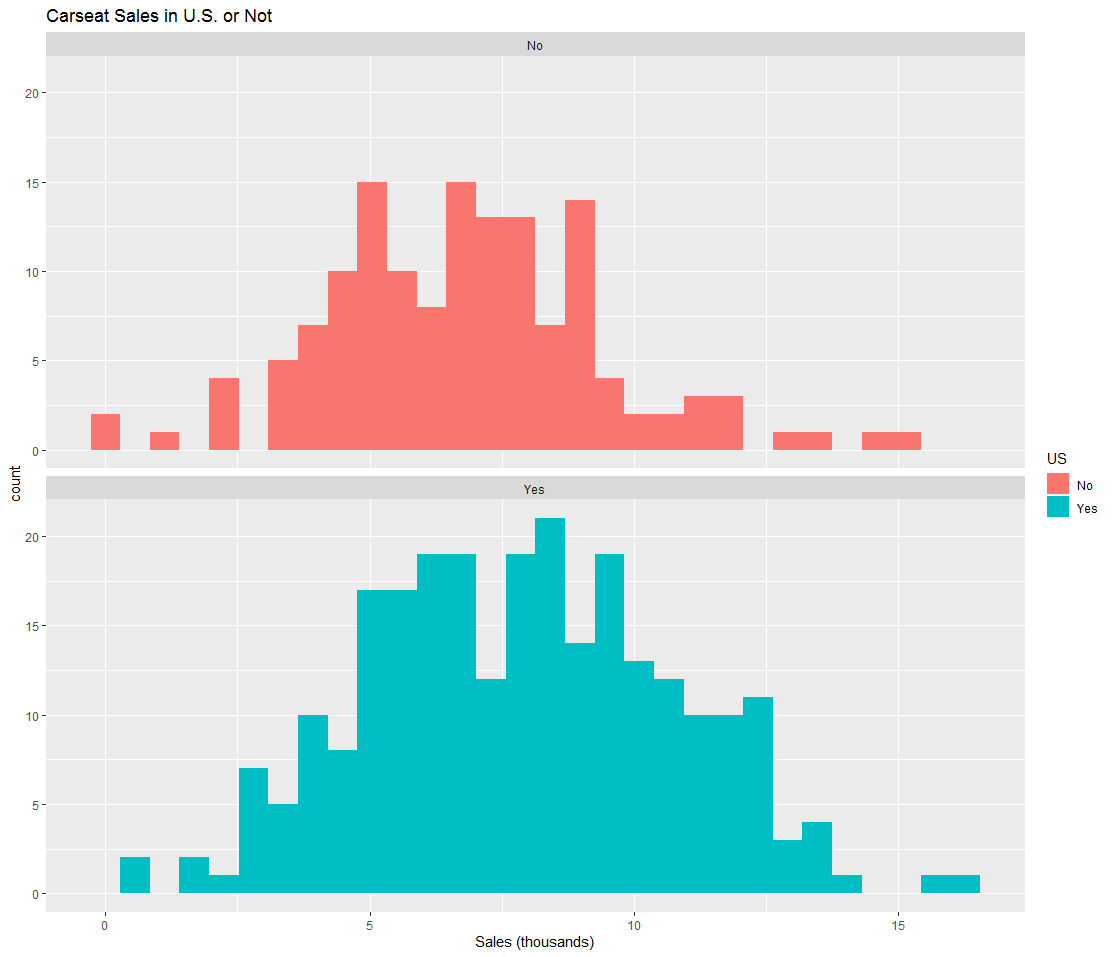
\includegraphics[width = 3in]{SalesUSHist.png}
\end{center}
\end{frame}

\begin{frame}
\ft{Does being in the U.S. change our Sales prediction?}
\begin{center}
	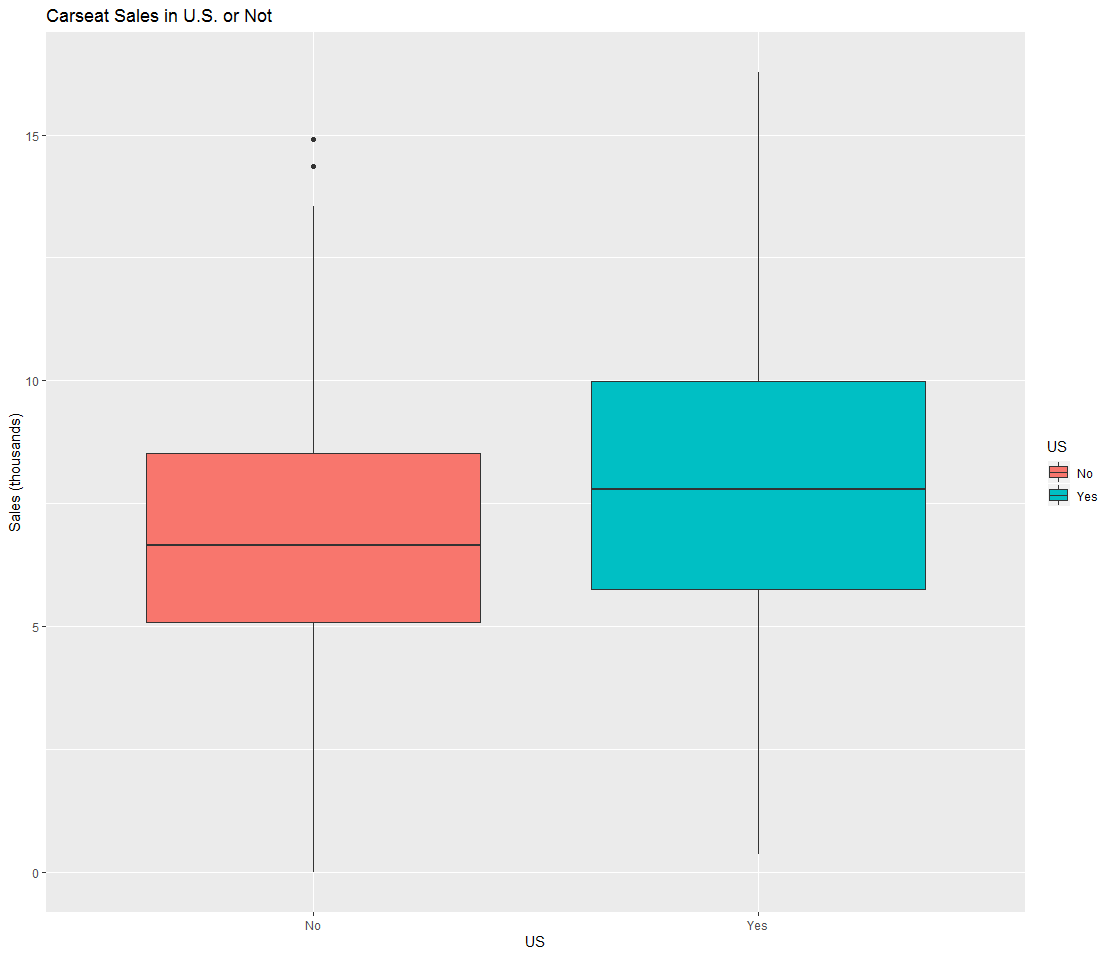
\includegraphics[width = 3in]{SalesUSBox.png}
\end{center}
\bi
	\item Any better?
\ei
\end{frame}

\begin{frame}
\ft{Predicting Sales Part II}
\bi
	\item If you knew a store was in the U.S., what would your prediction for Sales be?
	\pause
		\bi
			\item The most representative value of Sales for stores in the U.S. that we have access to, right?!
		\ei
	\pause
	
	\item The mean or average of Sales in the U.S. is a good start:
	\pause
		\bi
			\item Compute the average Sales for stores in the U.S.
			\item Compute the average Sales for stores not in the U.S.
		\ei
\ei
\end{frame}

\begin{frame}
\ft{So what did we just do?!}
\pause
\begin{center}
	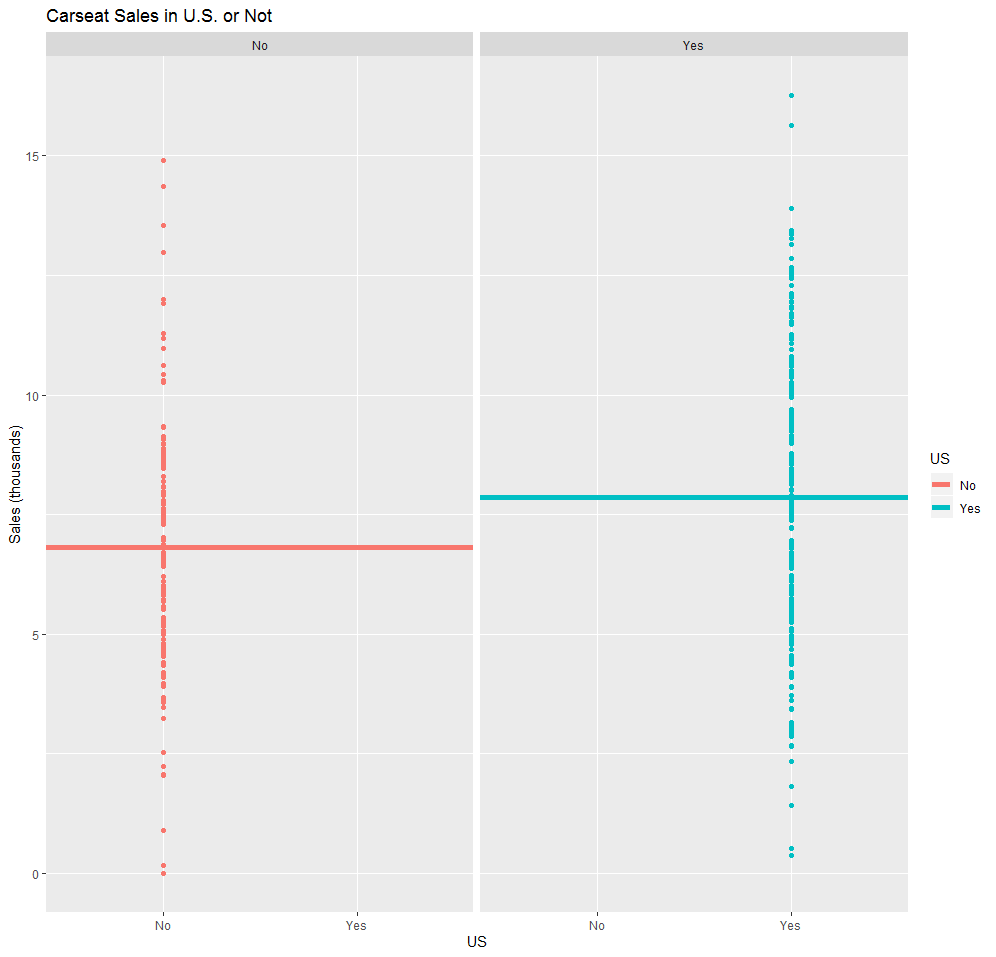
\includegraphics[width = 3in]{SalesUSPointsMeans.png}
\end{center}
\end{frame}

\begin{frame}
\ft{What are we doing \emph{\textbf{statistically}}?}
\bi
	\item Does knowing whether a store is in the U.S. change our prediction of Sales? \textbf{OR}
	\pause
	\item Is there a relationship between a store's location and its Sales? \textbf{OR}
	\pause
	\item Is there a difference in the average Sales between stores in the U.S. and stores outside the U.S.?
	\pause
		\bi
			\item Hopefully this last question sounds familiar...
		\ei
	\pause
\ei
\begin{center}
	\textbf{Two-sample ...}
\end{center}
\pause
\bi
	\item t-test
	\item confidence interval
\ei
\end{frame}

\begin{frame}
\ft{But What About the Lines on Those Graphs?!}
\begin{center}
	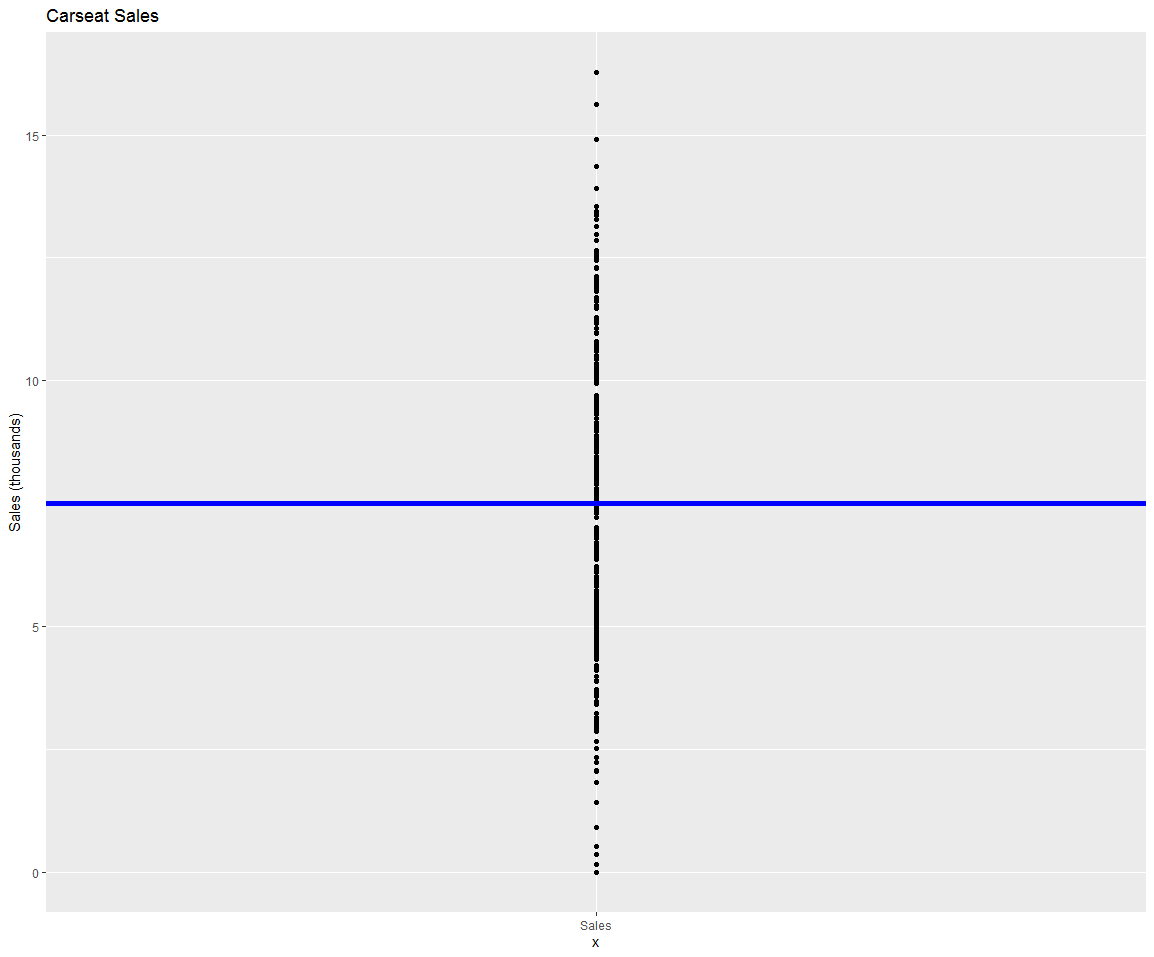
\includegraphics[width = 2in]{SalesPointsMean.png}
	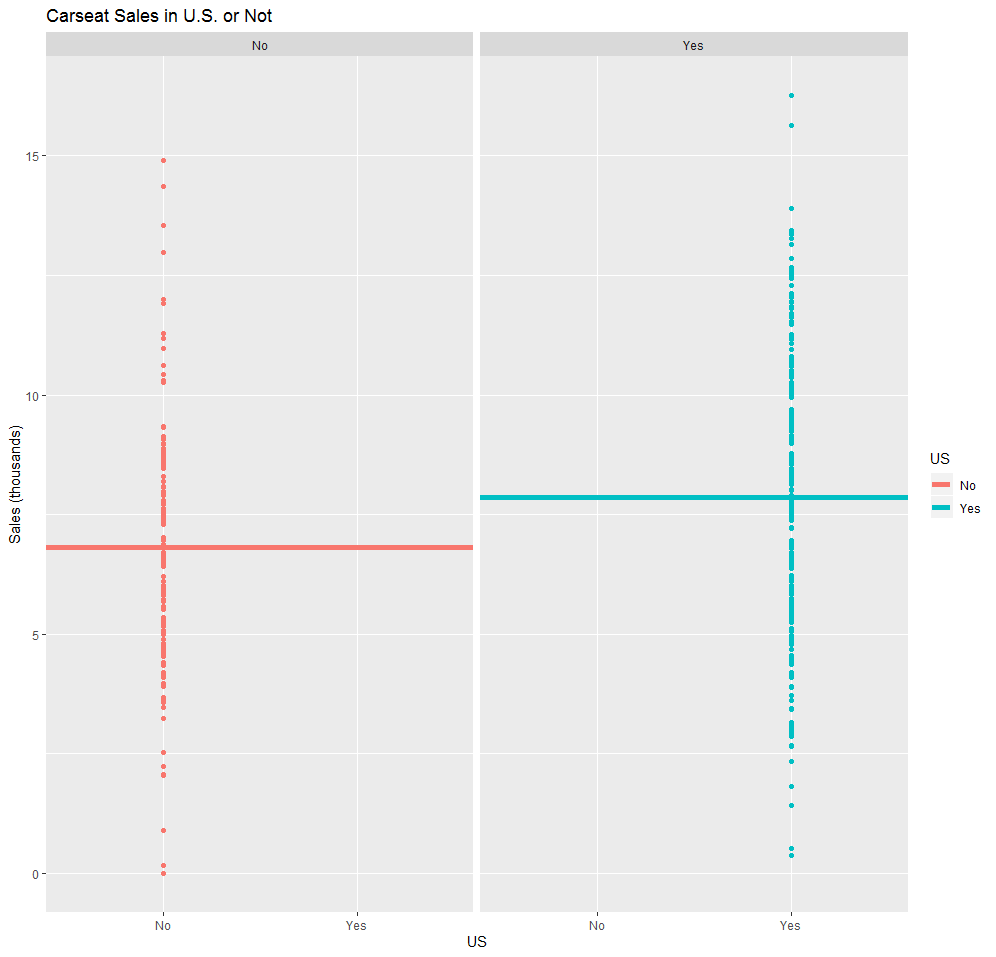
\includegraphics[width = 2in]{SalesUSPointsMeans.png}
\end{center}
\bi
	\item What's the equation of a horizontal line? 
\ei
\end{frame}

\begin{frame}
\ft{Our Models Thus Far}
\bi
	\item Sales alone:
	\[
		Sales = \beta_0 + \epsilon
	\]
	
	\pause
	\item Sales on US:
	\[
		Sales = \beta_0 + \beta_1 USYes + \epsilon
	\]
	
	\item where we assume $\epsilon \sim N(0, \sigma^2)$.
\ei
\end{frame}

\begin{frame}
\ft{Fitting Our Models Using Data}
\bi
	\item Sales alone:
	\[
		E[Sales] = \beta_0
	\]
	\[
		\hat{Sales} = \hat{\beta}_0  = 7.5
	\]
	
	\pause
	\item Sales on US:
	\[
		E[Sales \vert US] = \beta_0 + \beta_1 USYes
	\]
	\[
		\hat{Sales} = \hat{\beta}_0 + \hat{\beta}_1 USYes = 6.823 + 1.0439USYes
	\]
	
	\item We estimate the \textbf{\emph{average}} Sales using the fitted model!
	\item $\hat{\beta}_1$: we \textbf{expect} a 1.0439 thousand unit increase in Sales if a store is in the U.S.
\ei
\end{frame}

\begin{frame}
\ft{What is the relationship between Sales and Price?}
\begin{center}
	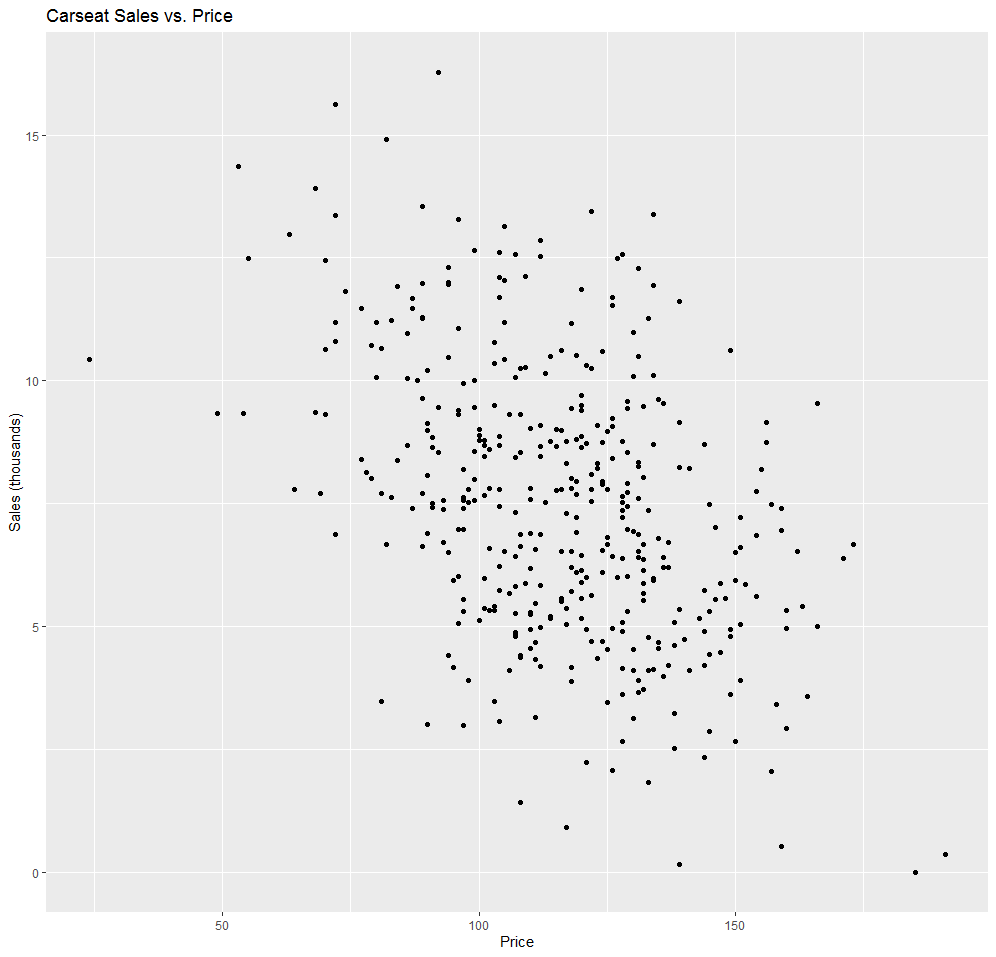
\includegraphics[width = 2.5in]{SalesPricePoints.png}
\end{center}
\bi
	\item How do we usually describe/interpret such plots?
\ei
\end{frame}

\begin{frame}
\ft{Correlation}
\bi
	\item What does \emph{correlation} measure?
	\pause
	\bi
		\item The \textbf{strength} and \textbf{direction} of the \textbf{linear} relationship between \textbf{two quantitative} variables.
	\ei
	\item What are the possible values correlation, $r$, can take?
	\pause
	\bi
		\item Between -1 and 1
	\ei
	\pause
	\item What else do usually hear about \textbf{correlation}?!
	\pause
		\bi
			\item \emph{correlation does not imply causation}
		\ei
\ei

\end{frame}

\begin{frame}
\ft{Can We Go Beyond Correlation?}
\bi
	\item What is your estimate of the correlation between Sales and Price?
\ei
\begin{center}
	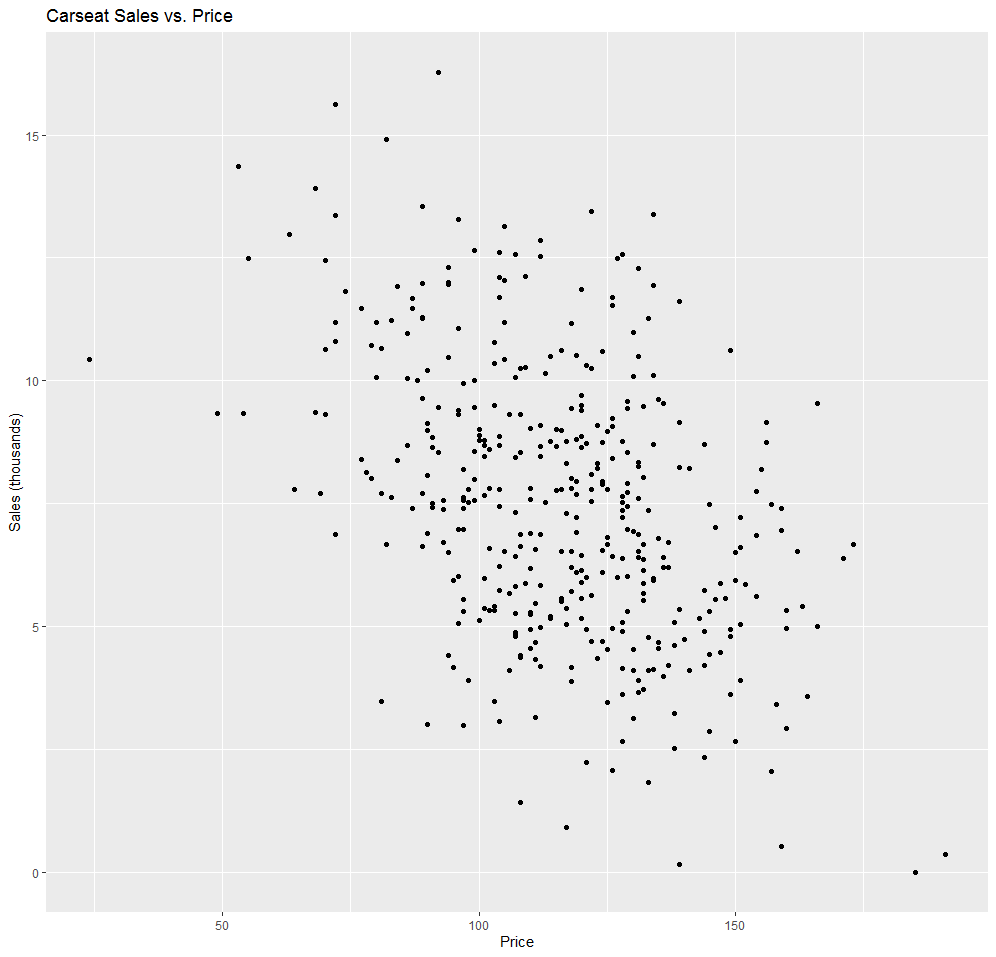
\includegraphics[width = 1.75in]{SalesPricePoints.png}
\end{center}
\pause
\bi
	\item $r = -0.445$
	\item How else could we describe the relationship between these two variables?
\ei
\end{frame}

\begin{frame}
\ft{(Least Squares) Best Fit Line}
\begin{center}
	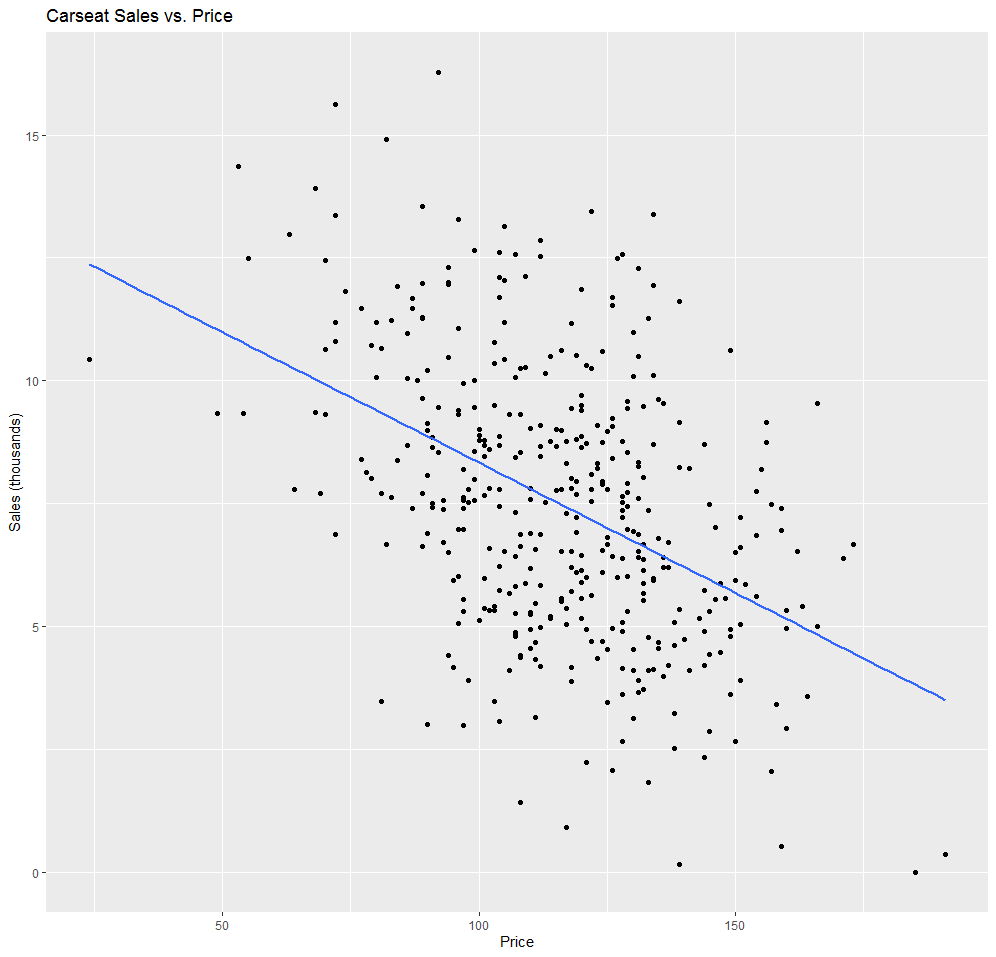
\includegraphics[width = 3in]{SalesPricePointsLine.png}
\end{center}
\end{frame}

\begin{frame}
\ft{The Model Equation of the Best Fit Line}
\bi
	\item Sales on Price:
	\[
		Sales = \beta_0 + \beta_1 Price + \epsilon
	\]
	\pause
	\[
		E[Sales \vert Price] = \beta_0 + \beta_1 Price
	\]
	\pause
	\[
		\hat{Sales} = \hat{\beta}_0 + \hat{\beta}_1 Price = 13.641915 - 0.053073Price
	\]
	
	\item We estimate the \textbf{\emph{average}} Sales using the fitted model!
	\item $\hat{\beta}_1$: we \textbf{expect} a 0.053073 thousand (53.073) unit decrease in Sales for every dollar increase in Price. (not causation!)
\ei
\end{frame}

\begin{frame}
\ft{Fitting Linear Models in R}
\begin{center}
	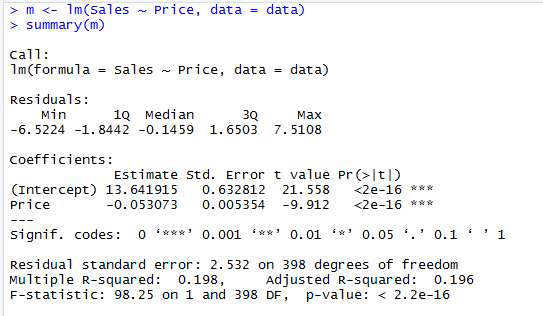
\includegraphics[width = 3in]{SalesPriceLMoutput.png}
\end{center}
\bi
	\item Check out the \textbf{estimate} column for the coefficient estimates!
\ei
\end{frame}

%\begin{frame}[fragile]
%\frametitle{Try It!}
%\bmp{1.0\textwidth}
%\footnotesize
%\begin{code}{.0}
%c(4, 6, 2)
%c("blue", "red", "green")
%rep(3, 10)
%\end{code}
%\emp
%
%\bi
	%\item We can combine things!
%\ei
%
%\bmp{1.0\textwidth}
%\footnotesize
%\begin{code}{.0}
%x <- c("blue", "red", "green")
%rep(x, 3)
%rep(c("blue", "red", "green"), 3)
%rep(c("blue", "red", "green"), each = 3)
%\end{code}
%\emp
%\end{frame}
%
%\begin{frame}[fragile]
%\frametitle{Sequences}
%\bmp{1.0\textwidth}
%\footnotesize
%\begin{code}{.0}
%seq(from = 0, to = 1, by = 0.1)
%seq(0, 1, 0.1)
%seq(0, 1, by = 0.1)
%seq(0, 1, length = 20)
%\end{code}
%\emp
%
%\bi
	%\item The \ttp{:} operator
%\ei
%
%\bmp{1.0\textwidth}
%\footnotesize
%\begin{code}{.0}
%1:10
%5:-5
%\end{code}
%\emp
%
%\end{frame}
%
%
%\begin{frame}[fragile]
%\frametitle{This....is....Vectorization!!!}
%\bmp{1.0\textwidth}
%\footnotesize
%\begin{code}{.0}
%y <- 1:5
%\end{code}
%\emp
%
%\bi
	%\item Square the values
	%\item Take the log of the values
%\ei
%
%\bmp{1.0\textwidth}
%\footnotesize
%\begin{code}{.0}
%y^2
%log(y)
%\end{code}
%\emp
%\end{frame}
%
%\begin{frame}[fragile]
%\ft{More on Vectorization}
%\begin{clicker}{What's the best way to add 3 to the values in y?}
%\begin{enumerate}
    %\item y[1] + 3, y[2] + 3, ...
		%\item y + 3
    %\item Use a loop
%\end{enumerate}
%\end{clicker}
%
%\begin{clicker}{What's the best way to divide the values in y by \ttp{6:10}?}
%\begin{enumerate}
    %\item y[1]/6, y[2]/7, y[3]/8, ...
		%\item y/6:10
    %\item Use a loop
%\end{enumerate}
%\end{clicker}
%
%\end{frame}
%
%%\begin{frame}
%%\fto
%%\bi
	%%\item Create a vector named \ttp{GPA} with values 2.9, 3.2, and 3.5.
	%%\item Create a vector named \ttp{age} with values 18, 20, and 20.
	%%\item Create a vector named \ttp{finanical.aid} with values FALSE, TRUE, FALSE.
%%\ei
%%\end{frame}
%
%\begin{frame}[fragile]
%\frametitle{Accessing a Vector's Elements}
%\bmp{1.0\textwidth}
%\footnotesize
%\begin{code}{.0}
%energy <- c(1894, 2050, 2353, 1838, 1948, 2528, 2568)
%\end{code}
%\emp
%
%\bi
	%\item We'll use square brackets to access vectors
%\ei
%
%\bmp{1.0\textwidth}
%\footnotesize
%\begin{code}{.0}
%energy[2]
%energy[c(2, 7)]
%energy[-2] \# all but 2nd element
%energy[-c(1, 2)] \# all but the 1st and 2nd elements
%\end{code}
%\emp
%
%\end{frame}
%
%\begin{frame}[fragile]
%\frametitle{\emph{\textbf{Which}} Position Can We Find Value \emph{\textbf{x}}?}
%\bi
	%\item Which position(s) equal 2050?
%\ei
%\bmp{1.0\textwidth}
%\footnotesize
%\begin{code}{.0}
%energy == 2050
%which(energy == 2050)
%\end{code}
%\emp
%
%\bi
	%\item Careful to use \ttp{==} to check equality and NOT \ttp{=}
	%\item A single equals sign (\ttp{=}) is another way to do assignment
%\ei
%\end{frame}
%
%\begin{frame}[fragile]
%\frametitle{Vector Referencing Using Booleans (TRUE/FALSE values)}
%\bi
	%\item We want to extract all of the values greater than 2000:
%\ei
%\bmp{1.0\textwidth}
%\footnotesize
%\begin{code}{.0}
%energy[which(energy > 2000)]
%\end{code}
%\emp
%
%\bi
	%\item The \ttp{which()} function here is actually unnecessary.
%\ei
%
%\bmp{1.0\textwidth}
%\footnotesize
%\begin{code}{.0}
%energy[energy > 2000]
%\end{code}
%\emp
%
%\end{frame}
%
%\begin{frame}[fragile]
%\frametitle{Side Note on Boolean Values}
%\bi
	%\item R treats TRUE values as 1 and FALSE values as 0
	%\item So, we can count things in a bit more clever way:
%\ei
%\bmp{1.0\textwidth}
%\footnotesize
%\begin{code}{.0}
%sum(energy >= 2050) 
%\# number of values greater than or equal to 2050
%\end{code}
%\emp
%
%\end{frame}


%===========================================================================================================================
\section[Multivariate]{Multivariate}
%===========================================================================================================================

\subsection{}

\begin{frame}
\ft{Our Dataset is Rich...Let's Use It!}
\bi
	\item Could we use both Price and US to help predict Sales?
\ei
\pause
\begin{center}
	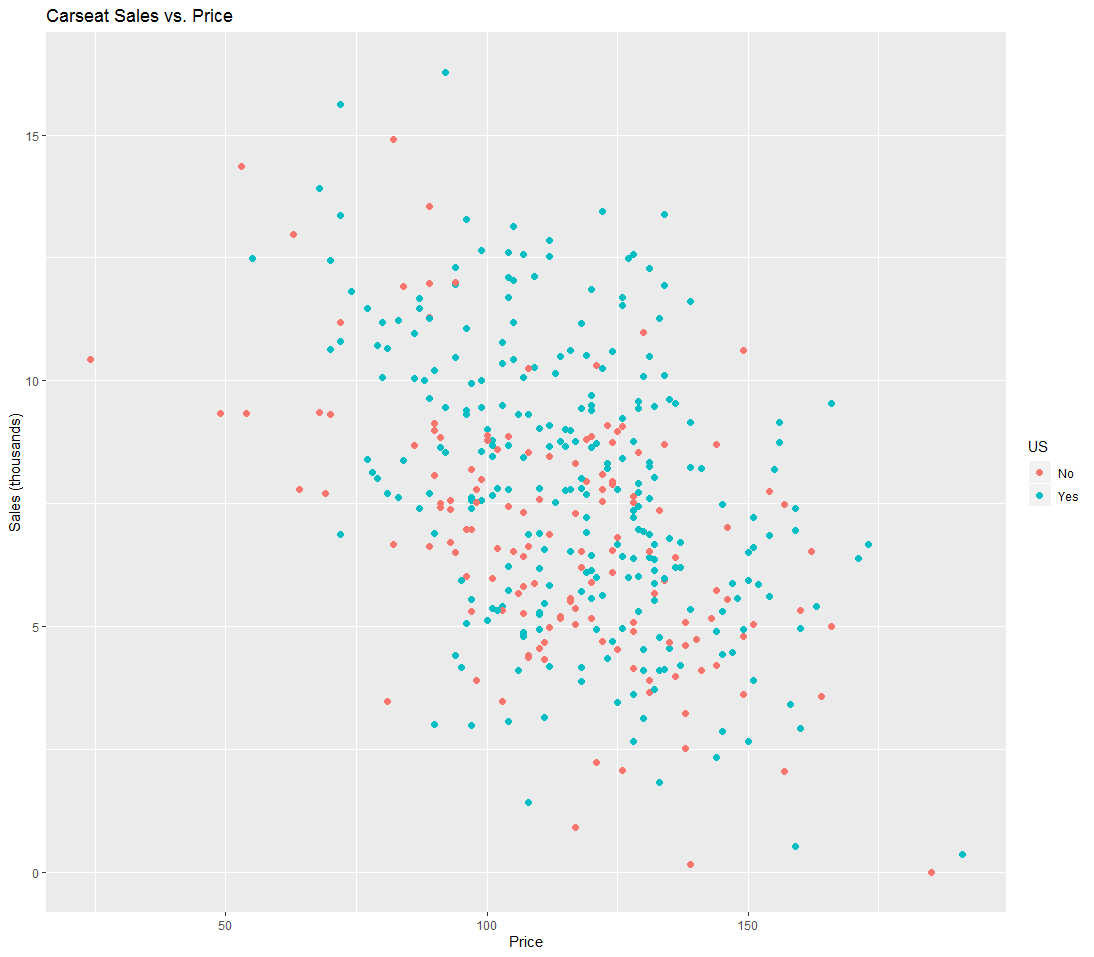
\includegraphics[width = 3in]{SalesPriceUSPoints.png}
\end{center}
\end{frame}

\begin{frame}
\ft{What Do We Do With Three Variables?}
\begin{center}
	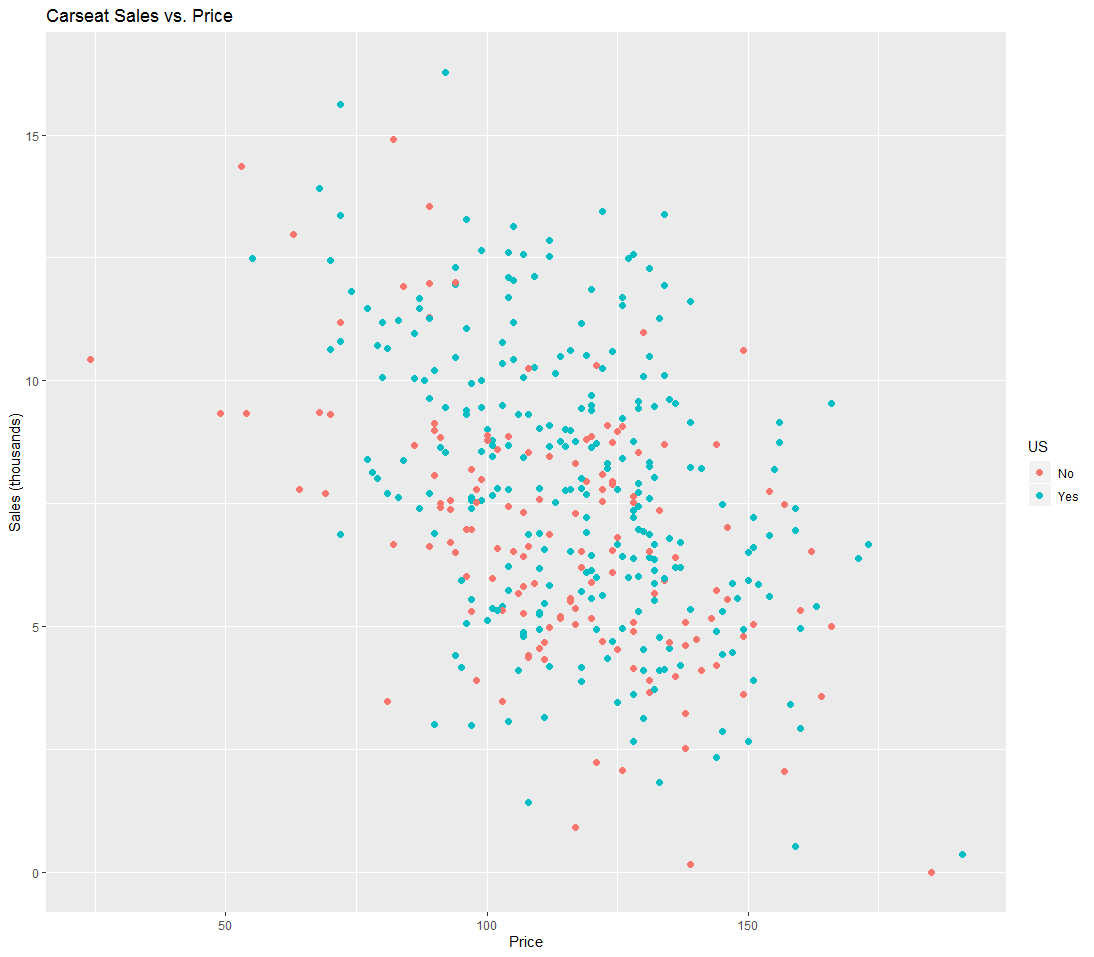
\includegraphics[width = 3in]{SalesPriceUSPoints.png}
\end{center}
\bi
	\item What are our model options?
\ei
\end{frame}

\begin{frame}
\ft{YOLO Lines!}
\bi
	\item We could allow for completely different fitted lines for each of the two groups:
\ei
\begin{center}
	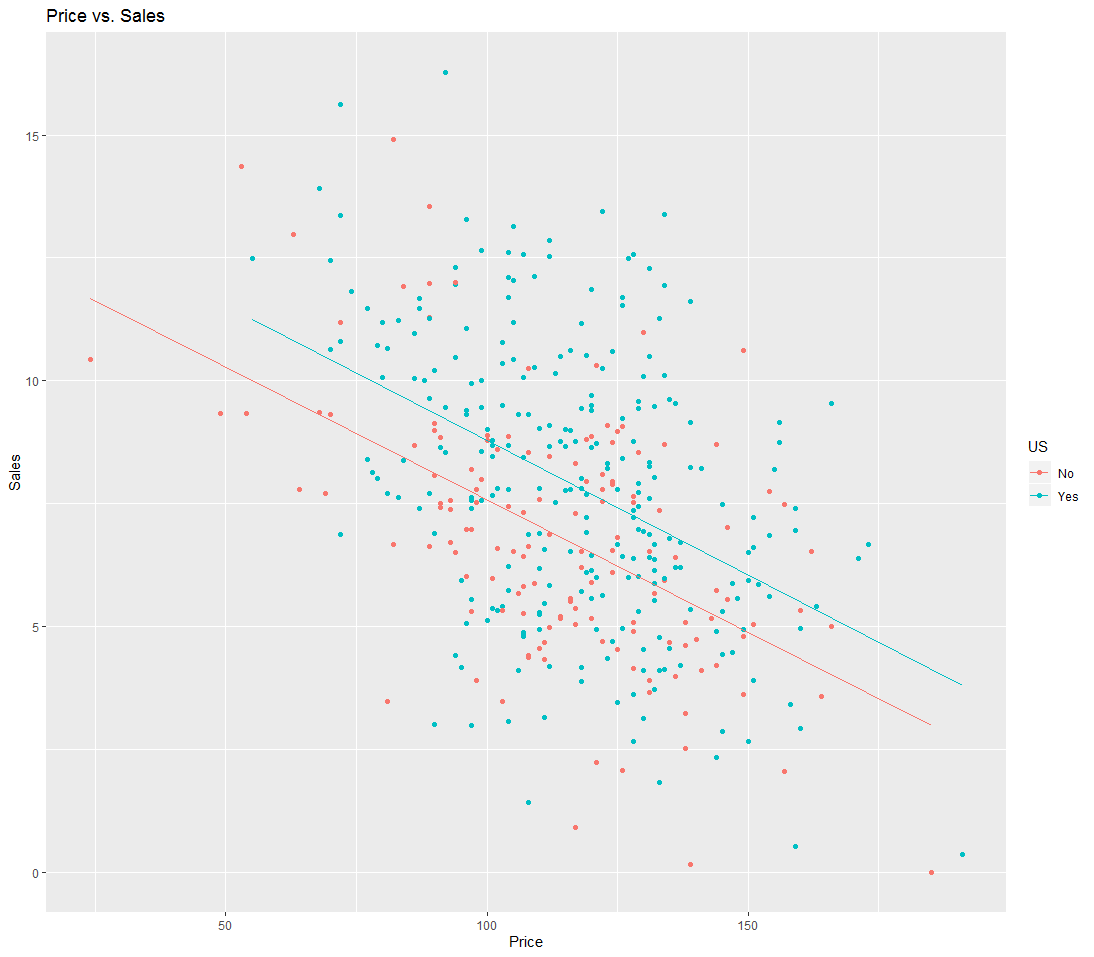
\includegraphics[width = 3in]{SalesPriceUSfull.png}
\end{center}
\end{frame}

\begin{frame}
\ft{Same Slope for Both Groups}
\bi
	\item We could force the line for each of the two groups to have the same slope:
\ei
\begin{center}
	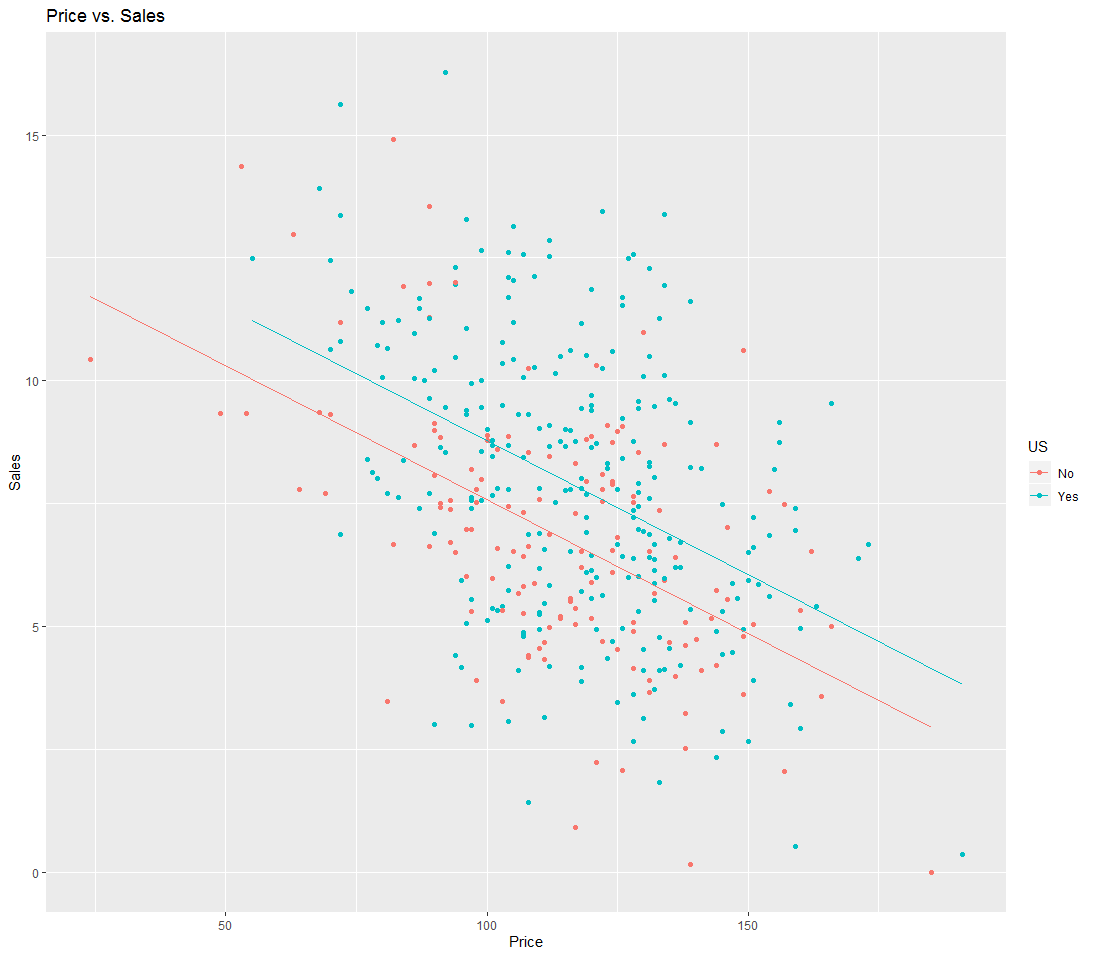
\includegraphics[width = 3in]{SalesPriceUSsameslope.png}
\end{center}
\end{frame}

\begin{frame}
\ft{Same Intercept for Both Groups}
\bi
	\item We could force the line for each of the two groups to have the same intercept:
\ei
\begin{center}
	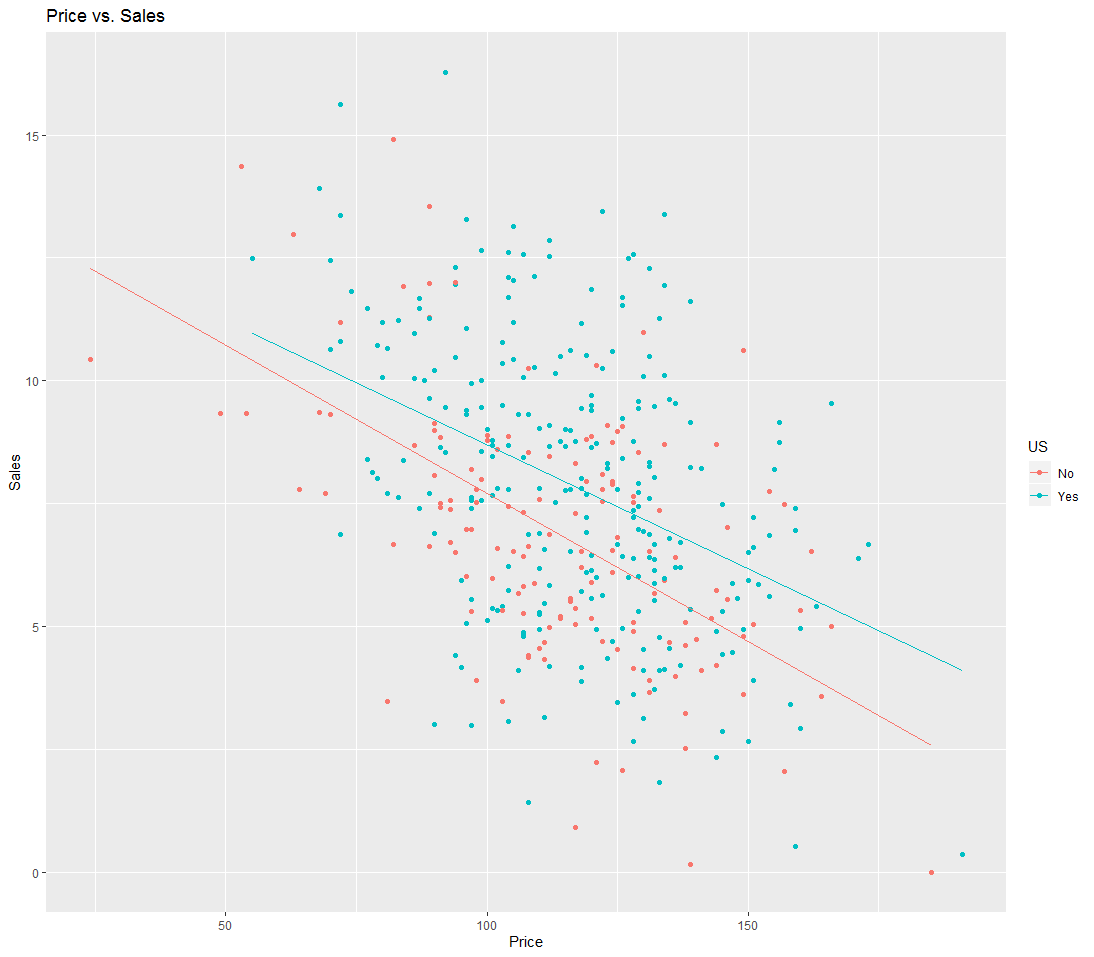
\includegraphics[width = 3in]{SalesPriceUSsameintercept.png}
\end{center}
\end{frame}

\begin{frame}
\ft{Fitting Bigger Models in R}
\begin{center}
	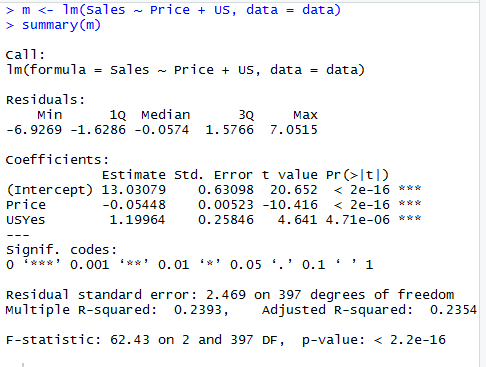
\includegraphics[width = 4in]{SalesPriceFullLMoutput.png}
\end{center}
\end{frame}

\begin{frame}
\ft{How do the interpretations change?}
\bi
	\item We could allow for completely different fitted lines for each of the two groups:
\ei
\begin{center}
	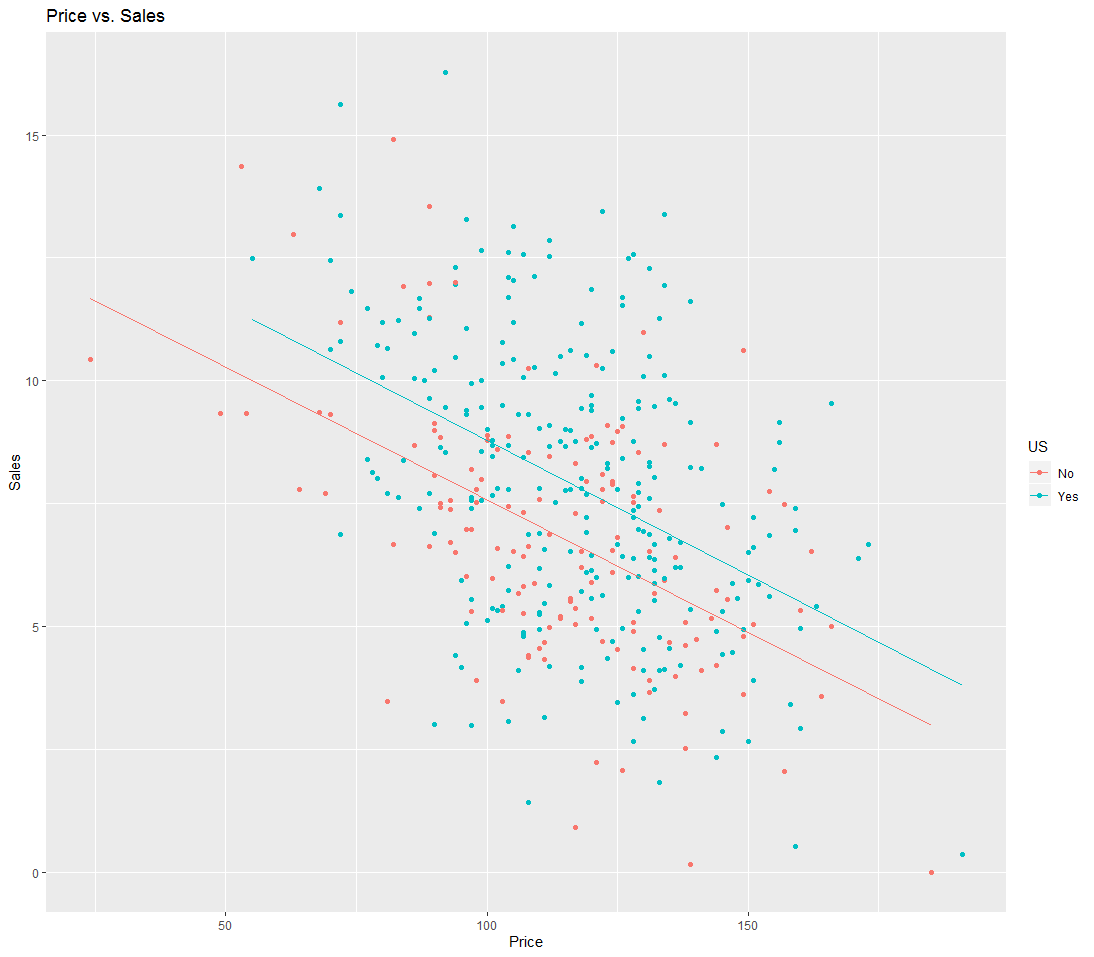
\includegraphics[width = 3in]{SalesPriceUSfull.png}
\end{center}
\end{frame}

\begin{frame}
\ft{We can get crazy!}
\begin{center}
	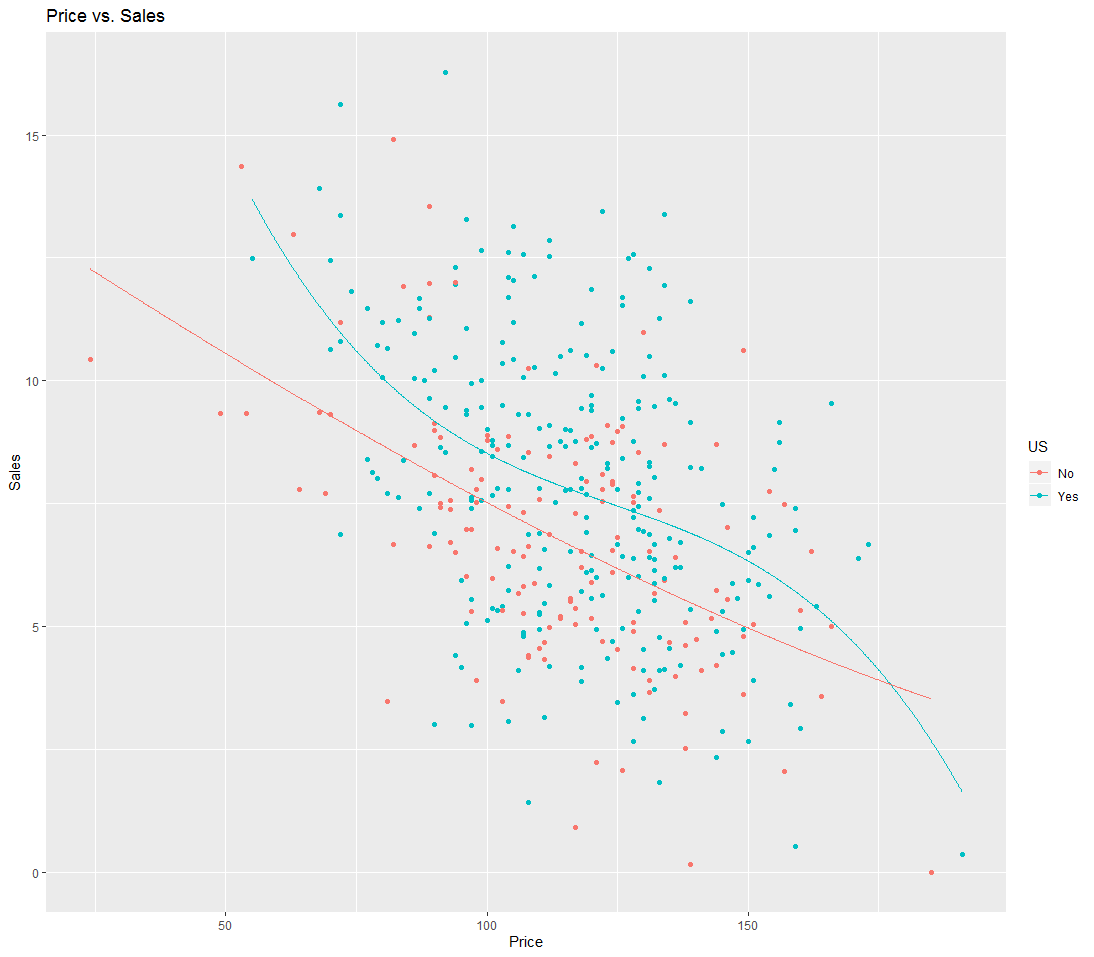
\includegraphics[width = 3in]{SalesPriceUSPoly3.png}
\end{center}
\end{frame}




\end{document} 